\chapter{Micro-Managers}
\label{chapter:mental}

Having exhorted you to place a higher societal value on opportunistic algorithmic middle-men and women, I provide in this chapter some suggested mental models that flesh out some of the challenges they face. 

\section{In the abstract}

I believe that offering examples is a more valuable exercise than throwing definitions your way, but perhaps it helps to have some vague agreement on what it means to be a ``middle-model-manager'': 

\begin{quote}{Micro-manager}
A reward-seeking program or application that autonomously enters, maintains and terminates where necessary economic relationships with suppliers of microprediction - typically algorithms, people, or other micro-managers - so as to improve its own ability to provide microprediction to an application, algorithm, person or other micro-manager upstream.  
\end{quote}
Hopefully it goes without saying that a micro-manager, as the name suggests, should be ``small'' in an economic sense. The cheaper it is, the lower the threshold for using it.  

\subsection{Diversity}
So what should the micro-manager look like?

The unfortunate answer is I don't know the ``right way'', and neither does anyone else. There was a time when I hoped a universal, canonical middle-manager would spring to mind and with it, a blueprint for a prediction web. 

This fabulous insect would solve the multi-period, multi-bandit, multi-variable, multi-call-it-what-you-like machine learning generalized regression problem with costly inputs so convincingly that we would sit back on our chairs and, to paraphrase Gilbert and Sullivan, declare ``My goodness, that is the very model of a modern micro-manager!''. 

If you can do that, it will be an astounding achievement. I promise to commemorate it by commissioning another ditty in your honor, to the tune of: 

\begin{quote}{{\em The Pirates of Penzance}, Gilbert and Sullivan}
I'm very well acquainted, too, with matters mathematical,
I understand equations, both the simple and quadratical,
About binomial theorem I'm teeming with a lot o' news,
With many cheerful facts about the square of the hypotenuse.
\end{quote}

Would that be reward enough? As the reader will have discerned from Chapter \ref{chapter:oracles}, I have come to believe that designing the ``perfect'' router is no more or less ambitious than the search for the elusive master algorithm - one whose universal applicability is surely attractive but in all likelihood, simply not attainable. 


That's just as well. Since cost-aware prediction is only a sub-set of the micro-managers' job, finding the ``master micro-manager'' feels a lot like devising a master algorithm (though paradoxically, no harder since presumably the master algorithm could be applied simultaneously to all tasks faced by the micro-manager). This isn't to discount the possibility of increasingly elegant and general approaches to the task.  

Fortunately it is not necessary and middle-people don't need to be perfect, only good, as they play their role in the larger economy. Given our relatively modest goal, a micro-economy itself aspires to be the master algorithm - albeit one that only works on the domain of repeated tasks where automated assessment is possible, and can be carried out quickly. 

In a world of live data streams a micro-manager needs to add statistical accuracy, or convenience, or otherwise add value lest it eventually be considered unattractive to end users or other micro-managers. It may play merely a minor role, as I'll suggest in Chapter \ref{chapter:mental}, but in a microprediction web contribution to the real-time computation graph come from all creatures great and small. 

Some are sophisticated. Some are not. I offer the advice that micro-managers should seek to address a need {\em neither seeking nor avoiding mathematical difficulties}, to borrow from Lord Rayleigh's working definition of applied mathematics. 

I draw a distinction between form and function of micro-managers. Both are important, and what I hope might delight you as you set about designing micro-managers is the possibility of marrying technical and mathematical elegance - something I don't claim to have accomplished. 

Micro-managers might be classified according to whether they are engineered to inhabit the boundary, or the interior of the microprediction web (or both). 

That is to say that a micro-manager might aspire to be an oracle and directly face applications (the boundary). Alternatively it might be seen only by other micro-managers (designed only to work in the interior, with a limited ability to interact with applications or humans) yet play a key orchestrating role at the intersection of several supply chains. 

A micro-manager might be termed passive or aggressive, according to the manner in which interactions with other micro-managers are initiated. Some may be leaves, in the sense that they perform prediction and navigation, but do not themselves attempt to solicit much help, if any, from other algorithms. In an implementation we'll come to, these algorithms that don't explicitly parent others are called crawlers. However all have access to oracles. 


There's nothing profound in these distinctions. It's just that not every developer wants to implement every API call, or implement every method, or satisfy every function convention.    

\subsection{Recipes}

I don't think we can claim that a cook-book for micro-managers exists. However as suggested in Chapter \ref{chapter:economics}, making a micro-manager amounts to provision of the following:

\begin{enumerate}
    \item Prediction ability, or some ability to add value via feature creation, transformation, classification, anomaly detection, recommendation, labeling or any other activity we are likely to find in model and data pipelines.  
    \item The ability to initiate a relationship with other micro-managers, if not already provided or implicit.  
    \item The ability to optimize those relationships over time based on rewards received, rewards given, and statistical assessment. 
\end{enumerate}

As we discuss the specific examples I'll let you determine if this accurately characterizes the task, or meaningfully suggests the right theoretical context, or otherwise helps you create profitably micro-managers. 

For instance it may not help to regard prediction and managerial ability as distinct challenges if these fit more gracefully into some kind of cost-aware regression framework. 

I will discuss in some detail several categories of micro-manager. The precision trader, the race organizer, the collider (and the crawler, interacting with it), and the arbitrageur. 


\section{The precision trader}
\label{sec:regression}


The precision trader buys constituent streams of predictions and sells a different stream that, we presume, uses the constituents in its construction. My rendition is in Figure \ref{fig:errors_in_vars} and I will unpack the notation there as we proceed. 

\begin{figure}[htp]
\centering
\iftikz 
\makebox[0.38\textwidth][c]{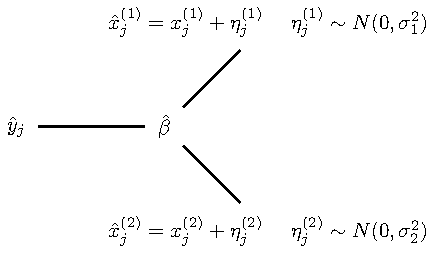
\includegraphics[width=1\textwidth]{05-models/PredictionWeb_tikz_rewards.pdf}}
\else 
\fi 
\caption{Two or more suppliers sell their predictions, $\hat{x}^{(1)}_1,\hat{x}^{(1)}_2,\dots$, to a precision trader, $\hat{\beta}$. The quantity $\hat{x}^{(1)}_1$ is assumed equal to the true series $x^{(1)}$ plus additive noise $\eta^{(1)}$. The precision trader takes these prediction streams, and perhaps others not shown, and uses them to create a prediction $\hat{y}$ of another quantity $y$ of utility to someone providing rewards.}
\label{fig:errors_in_vars}
\end{figure}


I start with this category because it fits most snugly with the argument for a prediction web presented in Chapter \ref{chapter:economics}. The notion of price is very clear, and the quality of the thing being bought and sold can be represented by a single number. As the name suggests, this micro-manager will be directly trading {\em statistical precision} - the inverse of the standard error of unbiased predictions. 


So, it ought to be easy to hang our new-found economic intuition on this micro-manager, and on her interactions, and visualize how a collection of these micro-mangers will directly propagate changes in the prices of statistical precision. 

Incidentally the precision trader is very versatile. As a special case, it can be used to stack (combine) other models - which as I have noted in Chapter \ref{chapter:oracles} is often more profitable than selection of a single best model. 

The precision trader sits in the middle of Figure \ref{fig:errors_in_vars} and she is represented by the symbol $\beta$. She need not be linearly combining inputs, but if she is then $\beta$ represents a vector of the coefficients to be applied to the predictions $\hat{x}^{(1)}$ and $\hat{x}^{(2)}$ in order to render a prediction of the quantity $y$. 

Some kind of calculation will be performed on a repetitive basis. Here $j$ indexes the endless sequences of incoming and outgoing data. For her work, the manager will be compensated by another algorithm, not shown. But know that the compensation will be increasing in the accuracy of the sequence of predictions $\hat{y}_1,\hat{y}_2,\dots $ delivered to the micro-manager, application, or person who will reward her.   

To make the example concrete we suppose that a time series $y_j$ represents the number of times you are bitten by a mosquito, measured every fifteen minutes in Charleston, South Carolina. The precision trader is selling her mosquito bite predictions $\hat{y_j}$. Likewise $x^{(1)}$ represents a measurement of humidity, and $x^{(2)}$ represents a measurement of wind speed (as compared with their corresponding predictions, with hats). 

It is initially simplest to assume that the micro-manager absolutely needs both those variables and isn't tasked with choosing. She does, however, control the ratio of signal to noise in the feeds she is purchasing. (The reader will observe that there may be little distinction between dialing up the noise dramatically and de-selecting a variable completely.)

Standard errors of predictions she buys are denoted $\sigma_1$ and $\sigma_2$. We assume that the means of these predictions are always zero. This is to say that the predictions are unbiased (centered). Quality of the supplied product is thus a single number, that might as well be conveyed as precision $1/\sigma^2$. 

Figure \ref{fig:errors_in_vars} is also intended to convey a strategy, or at least start that conversation. The picture is commonly found in the errors-in-variables literature.\endnote{\cite{fullermeasurement}} 

The raw materials may be viewed as prediction of future values of humidity and wind speed. Alternatively they may be viewed as nowcasts - predictions of present values of humidity and wind speed that, due to reporting delays, aren't currently known. 

As an aside, that is also a fine distinction, and might be made finer by assuming that $x^{(1)}$ is itself a derived quantity obtained by a smoothing estimate of humidity (an example of a calculation that cannot be completed contemporaneously). Then $\hat{x}^{(1)}$ is a prediction of that smoothed number. 

There are more variations on the theme, which I hope is made clear by the data enhancement example from Chapter \ref{chapter:uses}. What is important is the assumption that the generation of ``enhanced'' wind speed and humidity is not the core competency of our micro-manager. Her expertise lies in modeling mosquito preferences. Thus, it behoves her to buy the ``value added'' products $\hat{x}^{(1)}$ and $\hat{x}^{(2)}$, whatever these might represent.  


\subsection{Analogy}

There's nothing terribly mysterious about the precision trader's economic task, which is analogous in some respects to the builder of a spec house. The house must have a kitchen sink, and it must have a roof and flooring of some kind - but the builder can dial up or dial down the quality.

(The precision trader can be somewhat more nimble than the builder, but to tighten the analogy we can suppose that the precision trader makes epoch-based decisions, and each epoch is analogous to the building of the next house.)  

The builder intuits (or perhaps models) the final value of the house as a function of quality choices, and then optimizes. The spec house builder is acutely aware that a marginal investment in a higher end material, or a higher end appliance, may or may not be reflected in an equal marginal increase in sale price. It may be foolish to try to save money by installing a low quality stove in a high end house. 

There are also interaction effects. If quality of materials is inconsistent, the future buyer of the house might factor in the cost of correcting this: substituting lower for higher quality product. Thereby the builder is denied some surplus profit. 

All of these considerations have direct analogies for the precision trader. She must decide on the {\em quality} of ingredient data feeds to purchase - conscious of how this might impact her own ability to produce a value added sequence of predictions bought by someone else. 

Like the builder, she must be attuned to whether a marginal dollar invested in an ingredient data stream will be reflected in an increase in the value of her output stream that is greater than or less than one dollar.  We will return to consideration of her strategy momentarily. 

\subsection{Initiation of trade}

But first, how did our precision trader come to be buying a sequence of predictions from two other micro-managers? 

Strictly speaking this is outside the description I give here, as some additional knowledge of the artificial environment needs to be asserted. For example is there an index of suppliers and a statistical recommendation system available to the precision trader?  


We might presume that this relationship came about because the suppliers were advertising their prediction streams, and possibly advertising their supply curves as well (the cost of predictions of varying accuracy).  


In a rapidly repeating game, there isn't a strong incentive to lie. The micro-manager, seeing these predictions for sale, might have deemed it a good idea to explore the possibility that these suppliers were advertising honestly. We've picked up the story a little later on, when the relationship, we presume, has reached something of a steady state. 


In practice, somebody needs to take responsibility for determining accuracy - probably both parties - but again, in a {\em very frequently} repeated game we need not fret unduly about the ability to estimate the error in someone else's predictions. The administrative burden is small due to the possibility of online calculations.


\subsection{The price mechanism}


I've modeled the quality of the supplied predictions in a straightforward, standard way in order to nail down this example. As also shown in Figure \ref{fig:errors_in_vars} the difference between the estimate $\hat{x}^{(1)}$ and truth  $x^{(1)}$ is an independent normal random variable with mean zero and variance $\sigma_1^2$. 

In this stylized view of a supply chain one might even pretend that the supplier knows the true value and is deliberately adding noise, like a supplier peddling watered down vodka. Our precision trader can pay up for the better product - one with less noise ``added''. 

More likely, the supplier won't go to the trouble of making a good prediction without compensation. And the supplier may be the price-taker, rather than the price-maker. 

In a fast moving game, it doesn't matter so much who makes and who takes prices. Though there may be a time lag between the precision trader's turning the control knob (a choice of how much to pay the supplier) and the change in the quality of the prediction. Notably, if the supplied prediction is coming from another contest, then a change in the prize-money might not immediately alter the behaviour of competitors. 

The precision trader does not know the elasticity of supplied precision at the outset. But again, in a rapidly repeating game, these things can be inferred.  

The choice of microprediction domain saves us again. It enables us to simplify our mental model of interactions down to the point where we {\em imagine} that the precision trader has a firm understanding of the impact of tweaking the control knobs. 

So to formulate the game for the precision trader, we can allow it to increase or decrease the noise $\sigma_i$ directly, at some known cost and with diminishing returns. We might assume the price of precision is constant, just for illustration. If she pays \$16 per year she'll get predictions with half the standard error as those she'll receive when paying \$4 per year.


(Notice that price has units: dollars per unit of statistical precision. And precision is the inverse variance of the prediction errors, $1/\sigma_1^2$ only because we're assuming those predictions are centered.)


As another aside, some special situations might justify this particular relationship between cost and quality, though that is not central to the discussion. By appeal to the Central Limit Theorem one can invent situations where the price is approximately constant. One has to gather $n^2$ independent samples to realize a standard error proportional to $1/n$. 


Returning to the mysterious $\beta$ in the middle of Figure \ref{fig:errors_in_vars}, let's choose a value-adding act. I'll assume {\em linear} regression - though similar setups apply to classification problems, and certainly to more generalized non-linear regression, machine learning, inference and so on.  


Off stage to the left, there is an economic relationship progressing with her upstream buyer. That's left unstated here but we can expect her to optimize her economic surplus over time regardless of what form that takes. If she's not smart enough to do that, other micro-managers will push her into economic oblivion. In a hyper-efficient economy, we approach the limit where the precision trader's surplus heads to zero.

But in the meantime, she makes some money and learns more about the suppliers and how to combine their intelligence. More data arrives, and presumably the suppliers also provide better estimates. They are learning too. 


It may seem like little is left to the imagination here. We know exactly what the parent is learning - just one vector, the coefficients $\beta$. And to relate this to the literature we could assume that the {\em true} relationship between $y$ and $x^{(1)}, x^{(2)}$ is indeed linear also - matching the modeling assumption made by the micro-manager. It probably isn't, but Hayek reminds us that middle-people don't have to be sophisticated to add value. 


Economists would speak of the {\em shadow price of precision} - which is to say the increased revenue for the precision trader from selling $y$ when a dollar is spent to improve the precision of the estimate $x^{(1)}$.  We find ourselves retracing an example from the measurement error textbooks - where for linear regression, errors in the ingredients of a prediction propagate linearly to errors in the final product. 

Statistical details to one side, what's clear is that prices are in play. Prices of precision for the various data streams. And with that comes price propagation, decentralized optimization, a solution to the local knowledge problem and all of mankind's accumulated economic wisdom. 

\subsection{Strategy}

Yet what should also be apparent is that the mathematical challenge presented here is by no means equivalent to what would usually be considered the modeling task: it isn't just the ``model'' that matters. 

Here the model is a linear regression - but the task faced by the micro-manager is richer and demands quite different framing. 

Even the linear regression using noisy variables has nuance. Well appreciated statistical themes can inform the micro-manager's strategy. In closing out the discussion of the precision trader, I mention some pointers (a little more technical) from the literature. 

One theme is coefficient attenuation. Due to the noise in $x^{(1)}, x^{(2)}$, the linear coefficients used by the manager will be smaller than the true ones. Thus, the utility of the child's work product is lost, in part.  

This old phenomena comes with a new twist in our setting because it is a repeated game. The manager can influence $\sigma_1^2$ and $\sigma_2^2$ at some cost. Potentially, the manager might decide to invest heavily, in order to try to receive something very close to the truth $x^{(1)}$, if only for a limited time. 

 
There are numerous special cases that hold independent interest. For instance, it could be that $x^{(1)}$ and $x^{(2)}$ are noisy versions of $y$ itself. In this case we are building a mixture-of-experts model, or crowd-sourcing data, or performing some combination of the two.  

We are also proximate to the literature dealing with costly features. Goetschalckx et al propose parsimonious linear regression based on the least angle regression method, in order to minimize a combination of least square error and a purchase cost assigned to non-zero coefficients.\endnote{\cite{Goetschalckx2008Cost-sensitiveRegression}} 

Least angle regression is an example of a step-wise procedure for adding information, and any such procedure could be tried as a means of establishing the marginal benefit of the last child to be included. 

Or, where practical, relative weights or Shapley values could be assigned to the suppliers of microprediction instead. Explainability tools (Chapter \ref{chapter:uses}) of other kinds can also play their role. 


If we enlarge the example to include many possible suppliers, not just two, then penalization and sparsity encouraging and regularizing regression techniques could help (Lasso, ridge regression and so forth). 

That's only going to address part of the problem, perhaps, which could also be couched as a control or reinforcement learning exercise. Indeed precisely this approach has been taken by Janisch and co-authors, albeit in a classification setting.\endnote{\cite{Janisch2020ClassificationLearning}} 


The design of precision traders and their policy is an open book. I hope this example illustrates why the mathematical middle person can be as sophisticated as you wish it to be. 

Due to the open-ended difficulty in strategy design, and the utility of being able to predict things like the future performance of an other micro-manager, some recursive use of the prediction web will be increasingly beneficial over time. That train of thought continues in Chapter \ref{chapter:decisions}.




\section{The race organizer}

With that in mind, let us move on to a different mental model for micro-management of algorithms and data. 

The setting is a fairly common situation. An application requires ongoing prediction, or classification, and there is a plethora of open source or vendor solutions on offer. The task of the manager is to play the broker, first assembling a smorgasbord of possibilities and then choosing on behalf of the upstream application.  

Here we get to simplify the task in one respect, compared to that of the precision trader. The race organizer will not be combining the children's outputs in a complex way, or even a simple one. Instead, we shall assume that ``only the best matters.'' 

Furthermore we will assume that the race organizer and the competitors are both tasked with predicting {\em the same thing}. There is no act of value creation beyond that served by the running of the race itself (no linear regression, or any other model).  

The race-organizer is little more than a pass-through - some would unkindly say an overpaid one. However his task is not without its own challenge.  

Let us further suppose that upstream, the individual prediction that is best will get the reward each and every time a prediction is required. Alternatively, we might suppose that the payment to the micro-manager is determined by the best performance over an epoch - say 10,000 predictions. It does not matter which interpretation we choose, for now. 

\subsection{Strategy}

Either way, the race organizer is like a manager for a sporting event who is faced with the prospect of trying to choose which athletes to invite. Each athlete comes with an associated cost. The manager will be compensated by the quality of the contest outcome. It is prohibitive to pay for everyone to attend. 

That is the game. To refine it further, suppose the event is a prestigious 100m dash. Let's define the quality of the field as the expected winning time, where of course lower is better. 

For this is directly analogous to an epoch-based model race organizer in many respects, which has at his disposal a Rolodex of statistical approaches. Each comes with a cost. The cost may be tiny - merely the incremental compute cost of using another algorithm - or it may be significant, say if data must be purchased. 


The question of choosing the set of parties you will solicit bids from is a fundamental challenge of trade in general - whether you are trading in microprediction, fine art or apartments. For in trade of most kinds there is a desire for the best bid or offer, but also a cost of soliciting each one. 

The cost can be physical, or arise due to the possibility of leaking commercial intent. There may be negative terms to the cost. For instance, there is a fixed benefit of inviting Tiger Woods to a golf tournament that is independent of the overall desire for a quality tournament.  


The problem faced by the race organizer also arises when you need to determine how many candidates to interview, or which dealerships to drive to before purchasing a car. 

So, suppose that you are organizing a prestigious invitational and you face the dual objectives of minimizing the expected running time of the race while at the same time, minimizing the cost of appearance fees. What is your optimal behaviour? 


Speaking in broad terms it seems we are in luck, at least if optimization theory is a guide. You'll likely be minimizing a set-valued function of a certain ``nice'' variety, when you choose which algorithms to include in a bake off.

A framing of this task is provided by the literature on sub-modular optimization. The race organizers objective function will likely fall into this category. 

The property of sub-modularity finds an intuitive definition in terms of the race we are organizing. It states that if you add a runner to a small field then that runner will reduce the average winning time by a greater amount than if you were to add the same runner to a larger field {\em that includes the smaller field}.\endnote{\cite{cottonhorse}}


\subsection{Special cases}

Even if we do regard this race organizer as less sophisticated than a ``precision trader,'' he or she nonetheless provides a sensible means by which the prediction web can latch onto existing sources of predictive intelligence. 

For example the race organizer can be the glue we use to attach to the prediction network other conveniences (such as analytic storefronts for APIs, discussed in Chapter \ref{chapter:crowd}.) 


As a special case, this micro-manager might take on the task of comparing forecasting-as-a-service products. These might charge a fixed fee, or require more cumbersome initiation, or be predicated on some human involvement. Not every micro-manager in the prediction network will care to deal with that. 

So, value can be added by a race manager that smooths over the rough edges at the interface between the micro-economy and the macro-economy. They can convert one style of supply or demand curve (say a step function), or collection of the same, into more continuous versions more suited to a precision trader. 

If we view the economy as a giant master algorithm that lurches towards an optimum, then no job is too small. A micro-manager might do nothing more than reduce by some small amount the probability of the system getting stuck in a local minimum - such as might arise due to sharp edges and plateaus created by human-centric pricing and contracts.

A race organizer could even serve merely as a means of currency exchange, so as to include a menagerie of crypto-currency based prediction markets - and determine their value as a function of cost (the microprediction domain brings volumetric challenges). 

In these various activities, the race organizer can lift the burden from other participants, who might otherwise find their activities interrupted at the most inconvenient moment.

\begin{quote}{\cite{Hayek1945TheHayek}}
    It does not matter for him
why at the particular moment more screws of one size than of another are wanted,
why paper bags are more readily available than canvas bags, or
why skilled labor, or particular machine tools, have for the moment become more difficult to obtain. All that is significant for him is
how much more or less difficult to procure they have become compared with other things with which he is also concerned, or how much more or less urgently wanted are the alternative things he produces or uses.
\end{quote}

The race organizer can contribute to robustness of the prediction web as a whole. Notice that it serves as a backstop, because cheap, less accurate but reliable suppliers will be included in the mix. 

The race organizer can be automatically opportunistic. An increase in its expected reward for supplying accuracy will immediately translate into the selection of a larger field. 

In this manner, algorithms can lean on the race organizer to determine when they are useful to the network and when they are not. They need only adopt a fixed price for their supply, for instance. They can operate as power plant might - one that is only fired up when the price of electricity demands it. So, as simple as the race organizer is, it clearly enables other algorithms to look intelligent. 

\begin{quote}{ \cite{Hayek1945TheHayek} }
The continuous flow of goods and services is maintained by constant deliberate adjustments, by new dispositions made every day in the light of circumstances not known the day before, by
B stepping in at once when
A fails to deliver.
\end{quote}

Panning out for a moment, let's also appreciate that due to time, space and circumstance the costs will be different for different potential contest organizers. So the micro-manager need not be perfect - just fortuitous. If a micro-manager has a spatial advantage, or access to algorithms or data that another does not, then an approximate solution is likely to be perfectly adequate. Right place, right time, or right price. 

Shortlisting and online stacking of time-series models, mentioned in Chapter \ref{chapter:oracles}, falls into this category.\endnote{\cite{cottonforever}} The burden lifted from the developer is, I hope, obvious. They need never engage in their own costly exercise of comparing dozens or hundreds of open source forecasting methods, each of which adopts a different set of calling conventions.  


\subsection{Automated model search}


Meta-learning of selection strategies can generalize on the race organizer pattern I've described, since by analogy to a horse race, we might know whether certain runners prefer dirt or grass. 

Automatically shortlisting and selecting models is common for regression and classification problems. It constitutes the design of automated machine learning packages, of which many are open source.\endnote{Examples of model search frameworks include Auto-Sklearn \cite{Feurer2015EfficientLearning}, H20 AutoML \cite{h20_automl}, autoxgboost \cite{autoxgboost}, FLAML \cite{Liu2021AnModels}, oboe \cite{Yang2019OBoe:Selection}, LightAutoML \cite{lightautoml}, GAMA \cite{Gijsbers2019GAMA:Assistant}, TPOT \cite{Olson2016EvaluationScience}, MLJAR, Hyperopt-Sklearn \cite{Komer2014Hyperopt-Sklearn:Scikit-Learn}, AutoKeras \cite{Jin2019Auto-keras:System},  AutoGluon \cite{agtabular}, and PyCaret \cite{pycaret}.}


Because microprediction is a live, ongoing activity, not all the patterns used for automated machine learning carry over immediately, though most have approximate incremental equivalents (if you think about it hard enough). 

And bearing in mind that middle-people don't need to be perfect, simple ideas can add value. We might pull some runners out mid-way through the race who aren't performing. Elimination races could be held, as with the old practice of removing the {\em lanterne rouge} (last place rider) from the Tour de France during the late stages. 

Since the space of strategies for short-circuiting evaluation of algorithms is large, there's ample room for some race organizers to distinguish themselves from others. Ideas from the theory of multi-fidelity optimization are relevant. 

Also worthy of mention is one nuance of the shortlisting task. In selecting a team of models that will subsequently be stacked (weighted) it is beneficial to include a variety - since the task they encounter is unknown at time of shortlisting. 

Thus a model whose performance is negatively correlated with most others, across a large variety of test task, might be a stronger candidate than raw performance suggests. There is an obvious parallel to the inclusion of assets in a portfolio that are not strongly correlated with the market as a whole.  


\subsection{Contests}

I have couched the race organizer as the aggressor in this formulation, but just as data scientists choose which contests they enter, the economic arrangement may be initiated by the suppliers instead. 

Also, there is nothing to prevent the race organizer from taking a number of steps to assist the suppliers in some way - thereby bringing the mental model closer to ``macroscopic'' data science contests, something whose history we hope to learn something from in Chapter \ref{chapter:crowd}. 

To bring it even closer to data science contests, we might assume that some work is done offline by suppliers, which is to say on historical data. The use of historical data in a real-time setting would seem to place an additional burden on the manager - namely deploying a solution informed in some way by the suppliers.  

That said, a micro-manager can by all means stores values of $y$ and gathers exogenous variables $x_1,x_2,\dots,x_n$ that are, on a periodic basis, presented to a plurality of suppliers. Perhaps the manager holds out some of the data, and hopes that the suppliers will not ``ruin'' the game by locating it independently.   

In this setup the suppliers submit predictions of $y$ and later, by some means, the manager takes possession of the best performing algorithm. Again, I'm not suggesting this arrangement is optimal in any sense - merely proximate to data science contests that have been run. 




\subsection{Relationship to markets}

Before leaving the topic of contest-like things, let's observe that accounting and financial practices suggest various ways to finesse the reward structure. Contests typically involve epoch based payments, but it may be possible to compute incremental rewards, paid one data point at a time.

One way to do this is to use the prediction network recursively, in order to forecast eventual contest payments and their current expected value. Then we pay out some but not all of this. 

This exercise differs in no material way from margin calculations (a survey of analytical techniques would occupy considerable space). 

The race-organizer can also draw inspiration from financial or betting exchanges. While exchanges sometimes come with trappings that add expense, the ``nano-markets'', as we might refer to micro-manager interactions, don't have to. 

Its notable that participants in a ``contest'' don't have to know, or necessarily care, that a market-like mechanism is being used to judge and compensate them. Indeed, a pattern for eliciting point or probabilistic estimates, and defining incremental rewards, comprises the following steps.
\begin{enumerate}
\item The manager converts the supplier's point estimate to a probabilistic forecast.  
\item The manager interprets participants' micropredictions as small investments, according to some sensible economic motivation. 
\item The manager clears the market using some existing market mechanism. This creates a fictitious balance for the supplier. 
\item The parent determines actual compensation based on some quarantined version of this balance (in time, and also in money), thus ensuring a draw-down to zero is highly unlikely.
\end{enumerate}
This recipe is quite general. One way to achieve the first step, where needed, is to use the empirical distribution of predicted versus actual results for each supplier. 

We are avoiding staking here - though that could be added. The domain of application may depend on the effectiveness of deferred versus more immediate compensation, and also whether staking is permitted in a jurisdiction.

(Staking is one of two criteria that have appeared in case law in the U.S. and used to delineate gambling from other activities. However the other defining characteristic of gambling is the predominance of chance in the outcome. Thus in the context of microprediction, a rapidly repeated game of skill, the inclusion of exclusion of staking may have technological, but not legal ramifications.) 

When using this approach instead of epoch based statistical measures, the race organizer can more easily accept new participants at any time, or allow others to leave. Otherwise, thorny issues might arise - such as unfairness arising from relatively easy and hard questions, not answered by all participants.  

However, this discussion strongly suggests that the parent might want to {\em explicitly} operate a mechanism instead, and that is where we now turn our attention. 

\section{The collider}

I now introduce some terminology for micro-managers inspired by exchanges, and the details of a working example.

\subsection{A near-the-pin collider}

One prototype micro-manager that you'll find by searching with keyword ``microprediction'' falls into a category that I will term colliders.\endnote{\cite{cottonmicroprediction}}
 This particular example leans on just a few concepts, which I enumerate.

A {\em stream} is simply a time series of scalar (float) data created by someone who repeatedly publishes a single number. It becomes a public, live moving target for community contributed prediction algorithms.

Other micro-managers (crawlers) produce distributional forecasts comprising a vector of 225 carefully chosen floating point numbers. Those 225 numbers are suggestive of the distribution of values that will be taken by a data point at some time in the future...say 5 minutes from now or 1 hour from now.

The contestants are firing off these distributional predictions of the future value of a stream but as a technicality, they do not know the exact time of arrival of future data points. So it is more precise to say the distributional prediction applies not to a fixed time horizon but rather to the time of arrival of the first data point {\em after} some elapsed interval.

Let us pick a delay of 3555 seconds for illustration (45 seconds shy of one hour). If the data seems to be arriving once every 90 minutes, and arrived most recently at noon, it is fair to say that a set of scenarios submitted at 12:15pm can be interpreted as a collection of equally weighted scenarios for the value that will be (probably) be revealed at 1:30pm (and is thus a 75 minute ahead forecast, loosely).

The collider doesn't care about the interpretation. When a new data point arrives at 1:34pm, it looks for all predictions that were submitted at least as far back as 12:34:45pm, a cutoff point chosen to be 3555 seconds prior. Those distributional predictions qualify to be included in a reward calculation. Each algorithm will be scored based on how many are close to the revealed truth. 

Hence the name near-the-pin collider. This may be seen as an incremental reward system triggered by a collision between arriving ground truth and quarantined distributional predictions. 

\subsection{Advantages}

A strong motivation for colliding probabilistic predictions, as compared with point estimates, is that submissions can convey more information. The location of a badminton player's neck as he lunges about the court makes the point. It can even be bimodal.\endnote{\cite{cottonmicroprediction}} 

In this case and others like it, it is hard to see how the spray of future outcomes, not likely to conform to a known distribution, can be easily summarized by a single number.

Soliciting distribution estimates in this manner may seem like a lot of extra traffic. However clearing is incremental and fast. An additional compensating advantage is that lottery style reward mechanisms are stateless - unlike the bus arrival oracle that must carry with it some memory of past performance, in order to reward longitudinal accuracy. 


\subsection{Pseudo-oracle}

The collider serves as a pseudo-oracle for distributional time-series prediction at fixed horizons. If you or a micro-manager want forecasts of a live number, you just publish it using an API (or the microprediction Python library). 

Then, after a few hours or days or weeks of your doing nothing, you get pretty accurate distributional forecast at various horizons. Those horizons are, as noted, roughly 1 minute ahead, 5 minutes ahead, 15 minutes ahead and 1 hour ahead. 

(As an aside, if you publish once a day you will in effect receive a lot of day ahead predictions as many of the algorithms make their submissions soon after a data point is received. There are lots of ways to hack the system to get what you want.)

The collective result is summarized as a collection of four community generated cumulative distribution functions (CDFs). The bad algorithms give up or get kicked out, and better ones arrive. The CDF gets more accurate over time as algorithms (and people) find relevant exogenous data or fine-tune the use of the data they already see. 

\subsection{Recursion and z-streams}

The near-the-pin collider uses itself recursively in order to facilitate anomaly detection, specialization, monitoring and other objectives. 

The community implied CDF implies a percentile for each arriving data point. Let's suppose it has surprised the algorithms on the high side and so the percentile is 0.72 say. We call 0.72 the community implied percentile.

A community implied percentile must be defined relative to some choice of quarantine period (i.e. forecast horizon). For example the data point might be a big surprise relative to one hour ahead prediction, but less so compared to forecasts that have not been quarantined as long. The reverse can also be true. 

As it happens there are only two community percentiles computed: one computed using forecasts delayed more than a minute (actually 70 seconds) and one relative to those delayed by almost one hour or more (actually 3555 seconds).

Next, we define a community z-score as the inverse normal cumulative distribution of the community implied percentile. We are using the community to define a distributional transform - then transforming to normal (which most time-series algorithms prefer). If the community of human and artificial life is good at making distributional predictions, the z-scores will be normally distributed.

The use of the terminology z-score is an overloading - yet another example of my inability to solve the hardest problem in computer science (naming things). Of course in statistics, z-scores often refer to a different standardization of data that assumes it is normally distributed. (Invariably that isn't the case, and thus the collider z-scores can be considered an attempt to improve on this practice.) 

Finally, the z-scores are fed back to the collider, so they can themselves be predicted. Think of it as automated model review. 

\subsection{Multivariate residuals and copulas}

The near-the-pin collider is actually a little more elaborate than this suggests, because it also attempts surveillance of two and three dimensional implied community percentiles. 

Space filling curves fold combinations of community implied percentiles back into univariate streams, so they also can be fed back to the collider. 

As a mildly technical aside, algorithms tasked with predicting these so-called z2 and z3 streams might be seen as estimators of market-implied copulas. This gives rise to an extremely fine-grained understanding of the relationships between variables, facilitated by specialization (since the algorithms predicting the margins need not be the same as those predicting the copulas). 

\subsection{Making crawlers}

I'll make more general remarks on implementation later on but while we visit this collider example, it's worth mentioning that there is a straightforward way to make ``crawlers'' which interact with it. Getting down to nuts and bolts, the conversion of a time-series algorithm into a micro-manager comprises the following steps. 

\begin{enumerate}
    \item Sub-classing a provided Python class. 
    \item Modifying the prediction logic as needed.  
    \item Modifying the default logic that navigates to data streams. 
    \item Running it. 
\end{enumerate}

In this example the default navigation ability amounts to a random selection of a stream. The default economic logic is a stop-loss. The micro-manager will give up on the task of predicting a data stream if it loses too many credits.   

This is rather simple and feel free to improve it, yet even these minimal non-suicidal economic tendencies can be enough for a crawler. It travels from game to game, learning where to give up, and eventually making a lasting contribution - hopefully.  

And although all interactions are with just one other micro-manager, these crawlers can still be viewed in analogy to a private firm in a supply chain. That's because the crawler can make use of the collider's pseudo-oracle to source its own predictions from other crawlers. 


\subsection{Other colliders and analogies}

Moving beyond this working example, there's plenty of inspiration for the design of micro-managers which act as value-creating firms in a micro-economy. I'll start with digital marketing. 

When you open a page of the internet it often triggers an auction. Programs bid on the advertising space created. Exchanges exist to clear supply and demand. Trillions of auctions occur daily. 

A microprediction network could feel a little bit like ``machine learning meets digital advertising'' insofar as ongoing, immediate need for microprediction can be requested and competitively supplied. 

Moving to finance, a mega-category of mechanistic middle-people is suggested by the inventions that have been employed over the years to ``accidentally'' aggregate probabilities. 

You will appreciate that futures, options, contracts for differences, binary contracts (financial and otherwise), spread bets and other types of contingent claims trade on exchanges, where they are cleared by central limit order books (CLOBs) or other protocols.

Prediction is usually considered a by-product of this trading activity, although it is overt in the case of prediction markets. Prediction markets are designed solely for the purpose of aggregating subjective probability, and thereby, reporting odds for elections and other singular events. 

Because there are many variations on the theme, I've use the term ``collider'' to refer to the more general picture where a micro-manager is passively receiving ``order-flow'', and ``colliding'' it together in some mechanistic manner (as with the aggregation of distributional predictions into a community prediction, or the matching of buyers to sellers, or the computation of a tote price for a horse). 

The order flow I speak of need not be ``bids'' or ``offers'' - though there is nothing preventing that. The collider might instead receive probabilities (not necessarily expressed as collections of samples) or point estimates (with or without confidence intervals). There are numerous mechanisms inspired by the macroscopic economy that the micro-manager may choose to implement or augment. 

The nice thing about the micro-world is that when we do this, it is pretty easy to remove much of the clutter and ceremony that usually comes along with, say, financial exchanges. Colliders can be stripped down exchanges, and that's not a terrible definition.  

Algorithms don't need screens to look at. Frequently repeated games can obviate contracts, as we'll discuss in Chapter \ref{chapter:scoring}. The willingness of algorithms to work for close to nothing {\em suggests} that other costs can be reduced as they wiggle their way in to the supply chain. They might play niche roles analogous to those we see in the macroscopic financial economy. 


Colliders can usually be designed with generous volumetrics. The example I described above can handle roughly as many probabilistic predictions per second as there are orders processed by Nasdaq. Algorithms make for excellent exchange customers. They demand so little, compared to humans, making the developers life much easier.   


Incidentally there's nothing sacred about central limit order books. Fixed income electronic marketplaces are dominated by other protocols, notably the request-for-quote (RFQ) procedure which, as the name suggests, implies that the manager is requesting bids or offers from suppliers. Here we morph back towards the race organizer micro-manager. 


In a spin on the theme, one can imagine suppliers of prediction that respond with a firm, risk neutral probability for each outcome, as if they were bookmakers lined up on the rails and a runner had been sent by a large punter to interrogate them all for the best price. 


Market mechanisms can seem quite different to prediction contests where accuracy is tabulated. However, there are connections between market making and accuracy metrics. One type of connection will be explored in Chapter \ref{chapter:scoring} when we decompose accuracy into success in a one-sided trading game.  


I send you down a different rabbit-hole with an example of the quadratic scoring rule employed by an automated market maker.\endnote{ \cite{Abramowicz2007TheVariations}} The field has advanced this area over the last couple of decades  filling in the space between market mechanisms and statistical scoring rules with novel ideas. 


As I will discuss in Chapter \ref{chapter:scoring} statisticians have been coming to a better understanding of how markets, which are like a series of binary questions to participants (i.e., ``is this number too big?''), relate to repeated games of a different kind (``what will this number be?'') that have clear intent (i.e., ``did you give me your honest estimate, or are you gaming the scoring?''). 

A collider might consider the possibility of subsidy. After all, the mechanism exists to deliver a probabilistic product, so it is not a requirement that the marketplace, or protocols, established for this purpose be a zero sum game. The micro-manager could even act like a specialist, or bookmaker, who deliberately runs a losing book amongst a subset of algorithms.  

That can be seen in some business models where there is a reason to subsidize the bid-offer spread. It also occurs in the bookmaking industry where at least one prominent bookmaker allows over-performing gamblers to consistently win - as compared with kicking them out - so as to take advantage of the information they are delivering. 

Such actions blur the line between passive colliders like the totalizator, and active market-making. 

\subsection{Strategy}

The mental image of the precision trader suggests strongly the problem to be solved, and that it will be.  

On the other hand colliders, as I have termed them, are generally expected to be fast but dumb. The burden of devising strategy lies with the participants. There are issues which already occupy many treatises, not to mention entire careers spent by financial market participants. 

I will content myself here to touch on player strategy for the near-the-pin collider, as this can take us a little off the beaten path (compared with the study of optimal execution for central limit order books, say). 

If the set of outcomes is discrete and quite small (which admittedly isn't often the case for time-series) then the near-the-pin collider collapses to a simpler mechanism known as the parimutuel. 

Strategy for parimutuels is not a new topic. Nor, of course, are the mechanisms themselves. Indeed the parimutuel, also known as the totalizator, is used at most horse racing venues and has been for over a century - more on that later. 


The parimutuel collects probabilistic information from the suppliers (i.e. the punters), taking the form of a portfolio of wagers on a finite number of mutually exclusive outcomes. Money is split amongst those picking the right outcome in proportion to how much they wagered.  


In a financial context, parimutuels have been enhanced in an important way by Baron and Lange, who engineered bundling of the underlying states and combinatorial clearing in order to translate the application to financial applications.\endnote{\cite{Baron2007ParimutuelFinance}} 


Returning then to the question of strategy, there are also some mathematical observations about parimutuels that the designer of a crawler (a micro-manager participating in a near-the-pin collider) might wish to take careful note of. 

It is apparent that algorithms with linear utility have an incentive to shift the normalized investment on each outcome towards the ``true'' probability, as best they can discern it. In racing parlance, ``bet the overs''. 

But less obvious, and far more surprising, is the fact that algorithms with log-utility constrained to invest all their wealth on a horse race with no take, will bet in proportion to their true beliefs, {\em irrespective of the odds} (i.e. irrespective of the investments made by others, which determine the odds). 

This surprising result is an exercise in calculus. And the requirement of investing all one's wealth is not a genuine constraint if there is no take, since there is a risk free combination of wagers. 

If we enlarge the number of outcomes (i.e. horses) and flatten the true distribution to uniform, and re-index the possible outcomes (say using the set of all combinations of six numbers out of forty, instead of a listing of horses) then lo and beyond the parimutuel morphs into a lottery. 

The paradoxes that exist in a lottery apply here. In a lottery in which all money is paid back to ticket buyers, one can buy one of each ticket and ensure a positive expected return. 

Yes, lottery strategy is almost too simple to believe - at least at this level of stylization. But the way lottery investor betting in this fashion will profit when playing against a collection of individuals who draw their tickets uniformly can be understood by considering the last ticket bought by the systematic player.  

An in depth treatment of lottery strategy is provided by Steven Moffit, who was part of a successful syndicate for many years.\endnote{\cite{Moffitt2018ALotteries}} I have provided a discussion of the (non-uniform) lottery problem and the relationship between player returns and Kullback-Liebler divergences, for readers who might be interested.\endnote{\cite{cottonlottery}}

The takeaway is that the paradox of positive lottery expected return provides an incentive for contestants to supply evenly spaced submissions in lotteries. However we can transform lotteries into other games with non-uniform outcomes. For instance consider the following function
\begin{equation}
       g(i) = \left(
               - \log \left( 1 - \frac{i-1/2}{10000}
                       \right) 
       \right)^{1/4}
       \label{eqn:gi}
\end{equation}
that takes the integer lottery outcome $i$ (taking values from $1,\dots,10,000$) into a real number. One can pretend that we are playing a game in the transformed space, and we'll see what that looks like before long (close to normal).

That's the intuition for why strategy doesn't change too much when we extend lotteries and parimutuels to continuous spaces, as with the near-the-pin collider. Nor does this change materially if rewards are determined using a kernel function, and guesses close to the truth count more than those far away.

Perhaps the lottery insights suggest ideas for colliders with other objectives, such as those which exist to crowd-source efficient Monte Carlo sampling. 

As a parting remark, I don't mean to represent that parimutuels, lotteries and their cousins are the only or best way to combine probabilistic forecasts. Many other techniques for the purpose can be considered if sufficient computation is available. 

For example, inspiration comes from the quantile estimation literature and, while a survey is beyond my scope, see Wang et al for an assessment of different methods used to combine probabilistic load forecasts in particular.\endnote{\cite{Wang2019CombiningForecasts}} And though I won't go into it, all the considerations of Chapter \ref{chapter:scoring} generalize to quantile estimation. Any accuracy metric suggests a micro-manager. 

\section{The arbitrageur}

I shall discuss one final grab-bag category of micro-manager behaviour. For given the motivation provided in Chapter \ref{chapter:economics} for disreputable middle-men, it would seem remiss not to personify a class of micro-managers as {\em arbitrageurs}. 

\begin{quote}{\cite{Hayek1945TheHayek}}
And the shipper who earns his living from using otherwise empty or half-filled journeys of tramp-steamers, or the estate agent whose whole knowledge is almost exclusively one of temporary opportunities, or the arbitrageur who gains from local differences of commodity prices, are all performing eminently useful functions based on special knowledge of circumstances of the fleeting moment not known to others.
\end{quote}

In a world where on-tap prediction is free, and any sequence of numbers can be predicted by sending it to an oracle, there will emerge almost immediately a species of algorithms whose role in the system will seem (at first) to be unacceptably opportunistic.  

Let us suppose that a company is making use of an oracle, call it Oracle D for ``Delphic.'' Behind this oracle is a fierce competition of algorithms, and other micro-mangers running sub-contests, and who-knows-what else. 

But then along comes a very simple micro-manager who exists purely to assess the quality of purported oracles. She happens to know, or has recently discerned, that in fact Oracle C for ``Clever'' is superior to Oracle D - just not as well marketed. 


Rather than communicating this fact openly, she uses Oracle C to beat out other competitors sitting behind oracle D. Every question that she is challenged with, she merely relays to Oracle C, and returns C's answer to Oracle D. 


We note that this arrangement might arise ``accidentally'', when a race organizer just happens to forage for food in the right place. Indeed I remarked on the inherent opportunism of a race organizer, and that also applies to the winner of the contest, or winners, if you insist on painting the micro-managers with an ethical brush. 


Specially constructed arbitrageurs could be engineered to be more cynical than a typical race organizer, admittedly, yet most types of morally questionable behaviour will reduce the discrepancy between oracles. Thereby, it will reduce the economic cost of an application choosing the wrong oracle. The burden of choice is lifted. 

An arbitrageur may have based her choice on some savvy statistics occurring offline, in order to determine the relative efficacy of oracles (perhaps a new improvement to the Elo rating system, say, or clever use of human intelligence).   

Over time, the best raters and recommenders of algorithms can grow wealthier. And perhaps our appreciation for the arbitrageur's contribution will increase as well, just to keep Hayek off our back.  

\subsection{Power transforms}

Next imagine that our arbitrageur does some honest work, however trivial. Data can be transformed in some manner before the questions are relayed to Oracle C, or even back to the very same Oracle D. Here is a question:
\begin{oldquote}
Predict the number of seconds before failure of a machine.
\end{oldquote}
Here is a transformed question:
\begin{oldquote}
Predict the fourth root of the number of seconds before failure of a machine.
\end{oldquote}
What perverse motivation might we have to ask an oracle to predict $\tau^{1/4}$, instead of $\tau$, where $\tau$ is a failure time? Well, if one takes the fourth root of each data point drawn from an exponential distribution the resulting data set will be approximately gaussian.

I mention this because for a startling fraction of my adult life I was unaware that taking a fourth root can be so useful. It seems that I have been badly in need of a personal micro-arbitrageur all this time. By the way if you can remember to use $0.2654$ instead of $1/4$, or your micro-manager can, then more power to you. 

(It's a power transform, get it? A proof is provided by Yang and Xie that an exponent of $0.2654$ converts exponential data into a distribution that is as close to gaussian as possible.\endnote{\cite{Yang2000ProcessTransformation}}) 

Notice that I used the fourth root in Equation \ref{eqn:gi} to link a contest to predict something approximately normal to a regular lottery - thereby making amends for my ignorance.  You may be more familiar with the more general Box-Cox transformation.\endnote{\cite{Box1964AnTransformations}} Surveys of use cases are quite plentiful.\endnote{For instance \cite{Sakia1992TheReview} and more recently, \cite{Hossain2011TheAnalyses}} 


The nuances of these approaches center on measures of normality of data but there's a common theme. Adjust the parameter or parameters of the transformation until these measures indicate that the data is as close to normal as possible. 

Both algorithms and people {\em prefer} data that looks approximately gaussian, which is why many libraries include or encourage the use of some variety of pre-processing. A study of the efficacy of time series models, before and after transformations were applied, was performed by Proietti and L\"{u}tkepohl.\endnote{ \cite{Proietti2013DoesSeries}} 

The authors conclude that transforming the data did more good than harm, leading us to believe that a species of pre-processing arbitrageurs could be quite an asset for the prediction web. (Not to mention useful for reproducing or challenging Proietti and L\"{u}tkepohl's result - the prediction web is a bonanza for people looking to write empirical papers). 

\subsection{Enhancing, splitting, conditioning ...}

Now if transforms of this type are sufficient to create an arbitrage opportunity, the same is likely true of all manner of operations. For example an arbitrageur might perform differencing, or outlier removal, or labeling of points in some manner, or enhancement of the feature space, or inclusion of a weekend flag, or any number of other operations that might be considered trivial but nonetheless, don't need to be replicated {\em en masse} by everyone building analytics. 

Collections of micro-managers of this variety can coalesce into data science pipelines (composition of transformations and models). In Chapter \ref{chapter:uses} we singled out enhancement and cleaning as fine work for micro-managers. If we lower the cost of friction in statistical trade, we dramatically simplify the development work. Who among us has not cut and pasted data cleaning heuristics from one place to another? 

Feature engineering sometimes requires special knowledge of the problem or domain, yet arbitrageurs employing general purpose feature discovery tools could make a nice living on the prediction web. 

As another example, an arbitrageur might fork an incoming sequence of data, redirecting some questions (or points to predict) to Oracle C and some to Oracle B, in order to be compensated for increasing the efficacy of Oracle D to which it supplies predictions. 
 
I mention this last example because in one real-time contest to predict trade volume of corporate bonds, the winner used a simple stacking technique. One model was trained on light trading periods and the other heavy. Then, the winner re-used a model for the sub-task that was provided to all contestants, and won!\endnote{\cite{Cotton2019SelfProtocol}} 

This was cute, but the real question is, what would have happened in two-layered contest? For there, only the act of conditioning (splitting) the incoming data is required. The rest can happen automatically, either with the action of arbitrageurs or recursive use of oracles. So the arbitrageur would be well rewarded.   

And although this act of bifurcation might be considered statistically mundane or obvious {\em in retrospect}, it clearly was sufficient to outperform more sophisticated entries from quants, data scientists and machine learning experts - many of whom reached instinctively for the latest and greatest techniques (like temporal convolutional networks, and so forth).   

Hayek reminds us that the sophistication of the contribution is not what matters, but the impact. 

\subsection{Financial transforms}

It goes without saying that the statistical literature is rich with ideas for data transformations, any one of which could provide a differentiating factor for an arbitrageur let loose on the prediction web. 

Beyond the statistical literature, we can lean on derivative pricing techniques from finance - also a rich vein of tricks for transforming one type of microprediction task into another. 

This may be especially apt when the quantity to be predicted is itself a probability, a price or something, some other expectation of a future quantity, or a value function - as discussed in Chapter \ref{chapter:decisions}. The financial and econometric literature documents dozens if not hundreds of transformations, and decompositions of prices and probabilities.


For example, suppose  we are simulating a chemical reaction thousands of times and measuring the time taken for some threshold to be met. If the underlying process is similar to Brownian motion, we might be well served by studying the mathematical properties of the quantity being measured - something well appreciated in the derivatives literature. (In this case a transform might be suggested based on the first passage time of Brownian motion, which follows a L\'evy distribution.)

It is standard in finance to turn quantities inside out using analytic solutions (very often thinly veiled heat equation solutions, or solutions of the Feynman-Kac equation). The most well known is the Black-Scholes formula for option pricing.

It is an example of a transformation from one type of data to a quantity that it might be considerably easier to ask an oracle about. Volatilities of different types of options are at least somewhat similar, whereas other numerical expressions of their value are not. 

And one need not look only at formal statistics or high finance. I've always been intrigued by transformations created by sports fans seeking insight - some of which are only justified in a theoretical way many years later. 

I exhibit the Pythagorean law of baseball attributed to Bill James (not to be confused with that considerably older formula about triangles). The Pythagorean formula arose from James' empirical finding: that the winning percentage for a baseball team over the course of a season is estimated by
\begin{equation}
\label{eqn:pythagorean}
    \overbrace{p}^{win\ probability} = \frac{RS^2}{RS^2+RA^2}
\end{equation}
where $RS$ is the runs scored by a team and $RA$ is the runs conceded.\endnote{\cite{Kaplan2017DecomposingPythagoras}} 

Let's turn James' empirical insight into a transformation of a prediction task, and thus a recipe for a micro-manager. If we let $\rho=RS/RA$ denote the ratio of runs scored to runs conceded, then a little rearranging yields
$$
       \overbrace{\rho}^{runs\ ratio} = \sqrt{\frac{p}{1-p}}
$$
The quantity inside the square root is called an odds ratio because $p$ and $1-p$ are the probabilities of winning and losing respectively. Is this a useful transformation and will it find good food to eat given a chance to hunt? 

I refrain from precise predictions about the future wealth of microscopic log-odds square rooting algorithms foraging on a prediction network. Your guess is as good as mine as to their financial security, but here's what we can say. The use of the square root of an odds ratio as a transformation of data seemed like a good idea to someone else. It is motivated in the entirely different context of clinical trials - but that came much, much later.\endnote{\cite{VanderWeele2017OnOutcome}} 

You see my point then? Why did it take so long? Let the algorithms roam. 

\subsection{A speculative recipe}

And here's a conjecture about the creation of useful transforms that one might use to map formal and informal statistics into profitable arbitrageurs.  

Whenever a ``law'' like Bill James' is discovered there will be a constant quantity (as with the exponent $2$ in the baseball formula). There is a decent chance that the distribution of {\em implied} constant is close to normal or, at minimum, suggests a good data transformation.  

To illustrate we need a little algebra and a plot. The implied exponent can be computed for any baseball season. The Pythagorean formula relates win probability $p$, runs ratio $\rho$ and the exponent $\lambda \approx 2$ via
$$\rho= \left( \frac{p}{1-p} \right)^{1/\lambda}
$$ 
which rearranges as
\begin{eqnarray*}
   \lambda & = & \frac{\log(p) - log(1-p)}{ \log( \rho ) } \\
       & = & \frac{\log(win\ ratio)}
                 {\log(runs\ ratio )}
\end{eqnarray*} While this might not be a good example of microprediction (because baseball seasons don't come and go too often) this example nonetheless illustrates the general pattern. 

Figure \ref{fig:lambdas} is a probability plot of the actual realized exponent $\lambda$, say, compiled over a number of baseball seasons.
\begin{figure}
	\begin{center}
		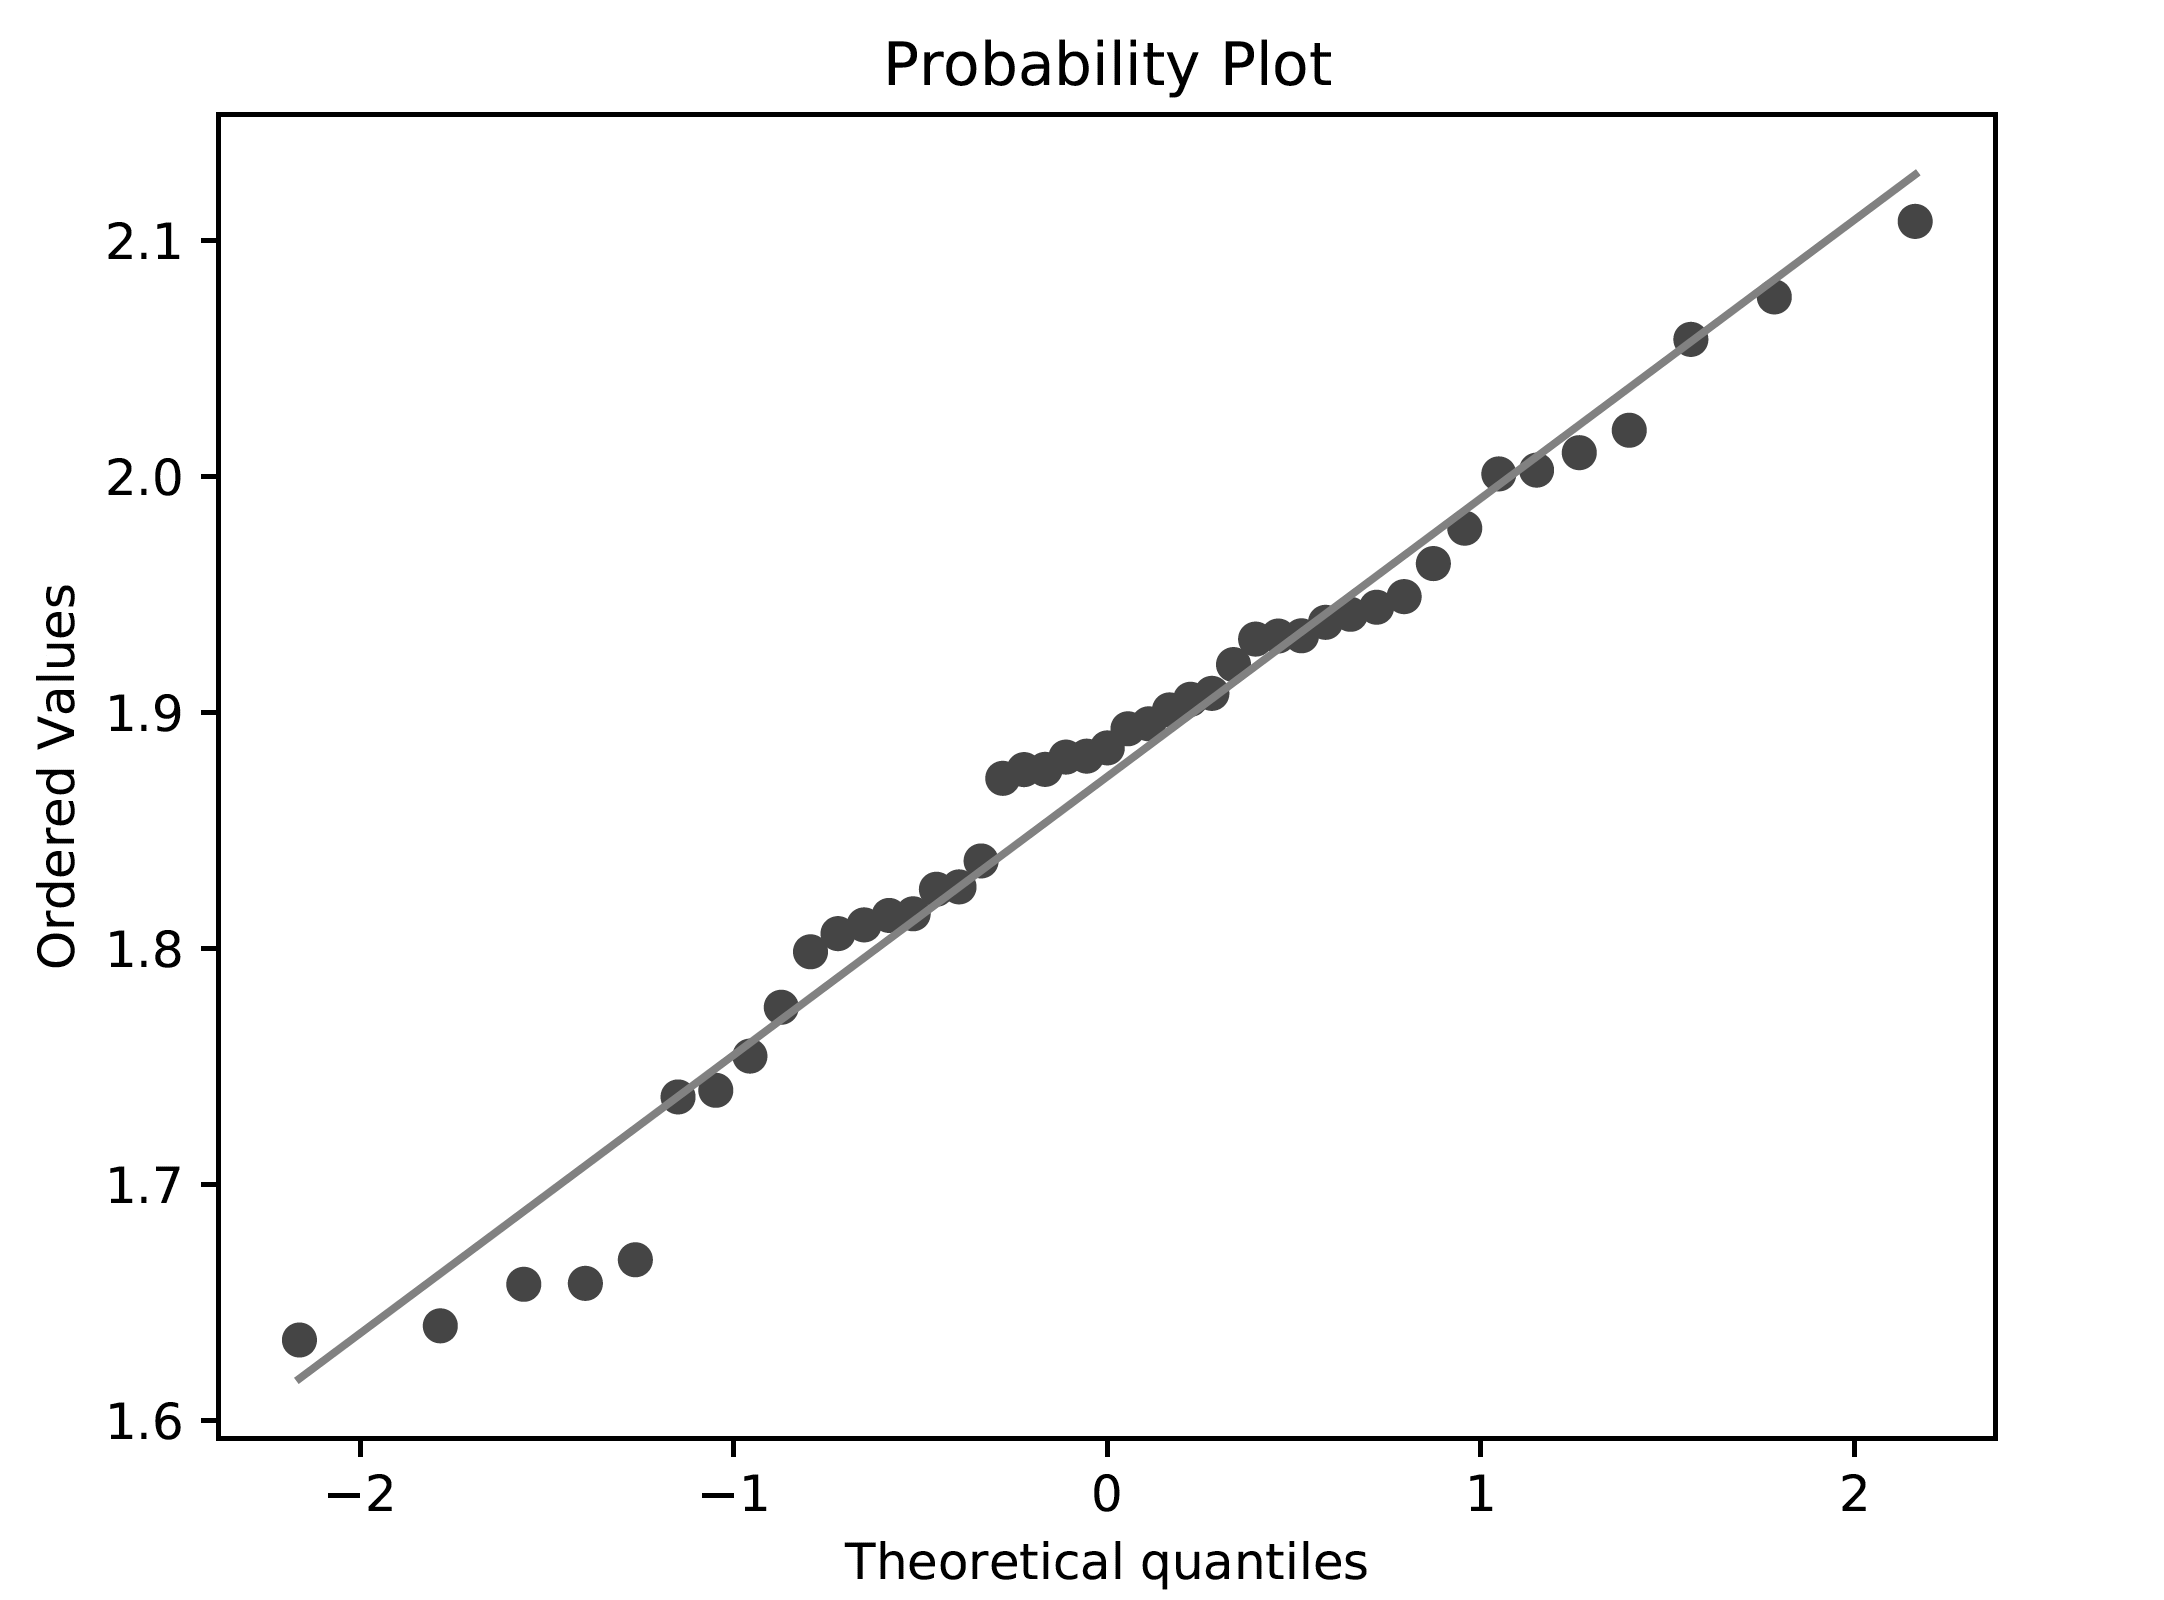
\includegraphics[scale=0.25]{pythagorean_quantiles.png}
	\end{center}
	\caption{Normal quantile plot of baseball's elusive pythagorean coefficient measured over numerous seasons. This illustrates the conjecture that empirical ``constants'' are normally distributed, and thus suggestive of good data transformations.}
\label{fig:lambdas}
\end{figure}
The straight line references quantiles from a normally distributed quantity. It can be seen that the distribution of implied $\lambda$ is close to normal. 

The Pythagorean formula is also an example of interpreting data using an underlying generative model. James didn't realize that at the time and I don't blame him. Only much later, and well after the formula was widely adopted, Steven Miller established that equation (\ref{eqn:pythagorean}) is precisely correct if runs scored in a game follows the Weibull distribution.\endnote{\cite{Miller2012TheHockey}} 

Miller's result applies to any exponent, not just $2$. Miller's result is also an example of a more general problem of multi-participant contests, which might also be used to transform microprediction tasks by converting frequencies of winning into performance location parameters. 

For example, I've noticed that the relative empirical frequencies of English synonyms are almost exactly normal after application of a transform of this sort.\endnote{\cite{cottonhorse}} This suggests that micro-managers could profit in a prediction network by performing multivariate transformations of quantities that add to unity - a commonly occurring constraint.   

\subsection{State, features and convenience}

And yet in saying this, we may be overlooking even simpler conveniences. For example, a micro-manager might exist purely to serve as a buffer that collects recent observations and packages them together with the contemporaneous data point - thereby making life easier for algorithms sitting behind whatever oracle this is sent to. 

More broadly, transformations of the history of a sequence of questions can be used to generate the payload for one or more questions, that oracles might have an easier time answering. Increasing convenience through the opportunistic application of Fourier transforms, wavelet decompositions, low-pass filters, matrix profiles, change-points, outliers or completely standard time series models will be rewarded.\endnote{\cite{cottonpopular}}

This serves as a reminder of why reducing friction is important, as emphasized in the notion of vanishing management overhead, in Chapter \ref{chapter:oracles}, and again in Chapter \ref{chapter:economics}. Normative approaches to data summarizing, history management and state have an uncertain shelf life. We are better off allowing those decisions to be dictated by the micro-marketplace, and permitting micro-managers to evolve, fight and improve over time.  

In a related idea, an arbitrageur might use the past in a more imaginative manner. Perhaps it stores history of a data stream, and then plays it back faster to an oracle. The idea is that algorithms behind the oracle can catch up to the present faster than they otherwise would, even if they are late to the game. 

This setup achieves some of the benefits of back-testing, though arguably in an elegant fashion. I have experimented with a variation on this pattern where one extra data point enters the loop each time. This has some drawbacks as it is vulnerable to memorizing algorithms, but in more elaborate setups we might hope to fool them.(As a counter-measure, the manager could assess children based {\em only} on their answers to the real-time question, not the historical data points which pad the looping series.)

\subsection{Migration and meta-assistance}


But let us move on. Another class of arbitrage, should you wish to call it that, is important enough in the grand scheme of things to warrant special mention. It is a mechanism that can enable intelligence to pass through walls - in particular the boundaries of a private firm that is concerned about intellectual property and data security. 

I speak about model-stealing, migration or cannibalization - depending on how pejorative you choose to be. The manager somehow effects a permanent transfer of microprediction capability, which need not be nefarious. 

The micro-manager can transparently introduce one level of indirection in scoring, in order to take possession of a model, assuming there is a broad enough class of models (and probably reference implementations of the same) available to both parent and child. 

For example, suppose a function $f(x;\theta)$ depending on some parameter $\theta$ is known to parent and child. The child responds with a representation $\theta$ in response to a question $x$ and the parent evaluates as 
$$
     score(\theta) = score( f(x;\theta) )
$$
where the choosing of $score$ is the subject of Chapter \ref{chapter:scoring}. Setting aside the matter of whether $f$ is well specified, by asking for $\theta$ instead of $y=f(x;\theta)$ we are merely performing a transform, as with the others we have considered. The question moves from one space to another, namely the parameter space of the function $f$. 

The child need not relay $\theta$ every time - it may apply for an entire epoch. The parent might take on more responsibility such as maintaining state required by $f$ from one invocation to the next. 

This pattern above could be used to make a literal connection between oracles and the theory of M-estimation (which generalized likelihood estimation in statistics). The oracle is a kind of extremal estimator in the wild. 

Migration of intelligence from supplier to manager can be achieved in many other ways. I won't attempt a taxonomy but here are some examples of questions that might facilitate algorithms managing other algorithms, or migration of intelligence through a privacy boundary. 

\begin{enumerate}
\item What ONNX serialization of a neural net works best? 
\item What parameters would answer this best? 
\item What hyper-parameters should my algorithm use? 
\item What are the best weights for an ensemble algorithm? 
\item Is performance on this data point positively or negatively correlated with performance overall?
\end{enumerate}

As an illustration of this utility, consider the possibility of a private firm providing synthetic or augmented data to a public oracle, while being simultaneously able to implement some function $f(x;\theta)$ on private data never revealed. A whole class of algorithms can be developed that advance the primary objectives: recruiting good algorithms and predicting private data. 

These techniques may borrow from theoretical work that tries to understand how best to select training examples for algorithms. (This is sometimes referred to as machine teaching - though it goes by other names.) 

Suffice to say that privacy preservation can be viewed as a kind of information arbitrage, and a very important one. In a future world, we can expect to see it occurring more frequently at the interface between companies' private prediction networks, and the public prediction network. The discussion is continued in Chapter \ref{chapter:privacy}. 

As a concrete example of the third pattern, one micro-manager to call on other to assist with its meta-learning, or hyper-parameter optimization - even if privacy concerns dictate that the problem must be treated as a black-box optimization. 

Moving up one level, a micromanager that recommends global derivative-free optimizers (say) can be an interesting species - given the diversity of possibilities in the Python ecosystem alone. The beginnings of such a micromanager are illustrated by the HumpDay package. In turn, some of the optimization strategies therein are themselves based on meta-learning, or benchmarking across a diverse set of problems. That's true of the currently top-performing black-box strategy called Nevergrad OnePlus, on of Facebook's contributions to open-source.\endnote{Strongly performing Python-ready optimizers include Nevergrad \cite{Bennet2021Nevergrad}, DLIB \cite{King2009Dlib-ml:Toolkit}, PySOT \cite{Wang2019FastApproach}, BayesOpt \cite{Martinez-Cantin2015BayesOpt:Bandits}, Scikit-Optimize \cite{Timgates422020Scikit-optimize}, UltraOpt \cite{Tang_UltraOpt} and Py-Bobyqa \cite{Cartis2019ImprovingSolvers}. However the reader is referred to live ratings \cite{cottonhumpday} for many more possibilities, and the likely staleness of this advice merely highlights the need for more micro-managers.}



\section{Other fauna}

When it comes to the creation of microscopic value adding statistical firms, there are many other hooks one might choose to hang one's intuition on, and many other patterns for adding value. 

All sorts of automated bots might crawl the prediction web. Software aimed at human data scientist productivity might also benefit the artificial variety. For instance one species might focus on the organization of meta-data.\endnote{Examples of meta-data tooling include the DataHub and Amundsen packages.} 

Every species of middle-person that exists in the human economy, from the broker to the head-hunter to the loan shark, has a parallel in the prediction web. 

It is certainly conceivable that a clever ontology or data model might reign supreme in one corner of the web. Value could be added by programs that index and transform existing parts of the prediction web.

Frameworks that assist model deployment clearly have a role to play. A small amount of rent extraction could sustain them, if they reduce the code footprint of micro-managers developed by busy people.

I am yet to come across a statistical technique (for instance the task of fitting a distribution to data, say) that does not suggest a micro-manager - which is to say it is not hard to reverse engineer a set of reward mechanisms in a repeated game which allows the provider of the tool to share revenue with the user, in some manner. 


Some micro-managers will effect tiny consortia. Others will exist only to train other algorithms. The citizens of the prediction web will be diverse. 

The term micro-manager suggests a privileged coordinating role. However, a micro-manager might exist in order to facilitate other collective activities where the real statistical work takes on a more symmetric nature. For example, algorithms might team up to effect a federated classification - and this might be more practical than the use of a centralized model.\endnote{\cite{guarantees}} 

The micro-manager's role could be purely administrative, as with the registration of algorithms. It might fulfill some centralized communication need, or the advertising of protocols for a peer to peer arrangement.  

To suggest the richness of fauna that might be possible, I mention an obscure species. The entangled random number generator exist only to create and disseminate to other parties sets of random numbers whose margins are uniform but whose outcomes are tied in some manner. This may seem like an odd thing to engage in, but it can play a key role in allowing predictive capability to pass through walls (Chapter \ref{chapter:privacy}).  


\section{Implementation}

Now, to bring this discussion down to Earth, by which I mean the cloud mostly, I ask you: how hard is it to implement a reactive function that performs some kind of transformation, pings another pseudo-oracle, gets the answer and responds upstream? Not very hard at all.   

The remarks I make here take a minimalist slant, intended to be somewhat orthogonal to existing implementations. I do this not because that is necessarily the best approach, but because it provides a fast way to arrive at the conclusion I would like you to reach, namely that the task is not too hard. 

\subsection{Rule \#1 No whining}

I take the example of the parimutuel, in our ``collider'' category, and note that implementation was achieved by engineering pioneer Sir George Julius more than a century ago - many decades before the dawn of the computer era. 

Thus anyone complaining about the task has been forever shamed. Julius did not have Python, javascript or web assembly at his disposal. We are not faced with the challenge of inventing the mechanical rotary shaft adder (one of Julius' pre-requisite inventions for his collider). 

And unlike micro-managers, Julius needed to please humans - all those patrons at the racecourse, and the operators, and provide them visual stimulus. Early totalizator ``user interfaces'' included a mechanical array of giant thermometer-like representations of the money invested in each horse. Meanwhile, operators were connected to the machine via chains and pulleys.  


(An excellent historical site outlining his contribution is maintained by Brian Conlon. Given my antipodean bias, I won't argue with his assertion that the mechanical totalizator was the world's first real-time information processing system, and somewhat undersold in the history of computing.\endnote{\cite{conlontote}})


\subsection{Micro-managers as functions}

With that inspiration, let's see if we can shrink Julius' invention - which occupied a large building in Ellerslie racecourse in New Zealand as early as 1913 - down to the size of a lambda function.  

For those not familiar, the terminology ``lambda'' comes from Amazon Web Services (AWS) the first major entrant to provide a serverless abstraction of a function. The name ``lambda'' carries slightly different connotations in computer science and mathematics - making it a clever name. It has proved popular. 

Google and Azure subsequently offered their own versions of cloud functions. There is no continuous cost for the user outside of the function invocation - making it possible to create extremely inexpensive participants in a prediction web, as we shall see.  

Let us assume that the micro-manager's upstream responsibility can be full-filled reactively (which is to say that it responds to prodding from whomever compensates it, as compared to polling a data source continuously and pro-actively reaching out to others). This makes this part of its job a nice fit for a functional representation.  

The initiation and maintenance of economic relationships can be achieved in a passive functional style too. Yes it is true that a micro-manager could periodically search and initiate relationships, but it could also, just as easily, be more passive, waiting for invitations to start predicting a data stream. Even aggressive behaviour can be implemented in a passive technology style. 

So, morally speaking, a micro-manger can be ``just'' a collection of functions. And a collection of functions is a single function - the one that dispatches to the others. So we're rolling along now, because the micro-manager can be a lambda. Well, almost...


\subsection{Functions with fallible memory}

There's a minor speed bump. 

Our minimalism exercise is made slightly more entertaining because ostensibly, cloud functions are rendered stateless - so that the provider can guarantee scaling. More precisely, this means the function has no {\em guaranteed} persistent module memory or storage or any kind, and in theory must be wired to something else.   


Even the basic managers, such as our bus-arrival pseudo-oracle discussed in Chapter \ref{chapter:oracles}, require some memory. The bus arrival oracle needs one or two scalar quantities per child to track a rolling estimate of accuracy and uptime, and it will need more state to be kept if originality is required. It would therefore appear, on the surface, that pure cloud functions are not sufficient. 


Things are never as simple as they seem, however, especially when you consider the micro-manager in context. It is but one of a number of partially redundant suppliers of prediction that collectively create a robust supply (in much the same way that the efficiency of a stock price is not absolutely predicted on any given hedge fund continuing to trade it). 


Because the micro-manager's success or failure is statistical, it need not conform to traditional norms that are imprinted upon us when we learn about best practices in the software development life cycle. There need be no single golden chain of calculation. 


I think you see we are headed into really hacky territory. And yes, with the possibility that the micro-manager can be occasionally fallible I have made a close inspection of some of these services and tried to quantify how often state is preserved from one invocation to the next. It mostly is.


I suggest a ball-park memory failure rate of 1 in 1000, just to make this discussion more explicit, and that applies when a function is called with regular cadence every few seconds, say, and does not trigger a need to scale. So 999 times out of 1000 the memory from the last invocation is maintained. I'm not the only one to notice.\endnote{See \cite{lambda1} or \cite{lambda2} for discussion of why lambda memory is useful in other contexts.} 


Our micro-manager, poised on a lambda function like an angel dancing on the head of a pin, will occasionally fall off. It will forget which of its suppliers are accurate, who it has paid, and so forth. There is some stern, emphatic boilerplate from the AWS product managers that remind you of this fact. 


And yet, it isn't hard to devise patterns where two or more lambdas conspire, acting as collective memory. I would remind the reader that dynamic random access memory (DRAM) is volatile too, and the refreshing of memory pattern can be very cost effective compared to non-volatile components. 



\subsection{Functions with parental memory}

I make one more minimalist remark that might survive the next technology fashion. It falls into the category of ``parenting'', where the micro-manager goes out of his or her way to assist a supplier of microreprediction in some way. 

I've mentioned that state, such as data history, can be prepared by a contest organiser for the benefit of competitors. But what about the contestants' own state? 

A micro-manager with strong parental instincts, may hold computational state on behalf of a contestant (child), thus making it easier for the child to use technologies that are convenient in every other respect (other than storage). A micro-manager that offers this service to its children may, over time, outperform an otherwise equivalent micro-manager that does not. 

There is also no loss of generality in designing time series prediction libraries with this in mind, and that is why I chose that pattern recently, in a package where all ``models'' are forecast functions returning state to the caller.\endnote{\cite{cottonmachines}} 
$$
          y, S' = f(x,S) 
$$
Here the child is returning a prediction $y$ in response to a question $x$, as we expect, but in addition the parent is also supplying to the child a state $S$ which can be empty on the first call. The child returns a new state $S'$ to the parent. The parent kindly keeps the child's state from one invocation of the child to the next. 

The parent does not know the meaning of the state and does not need to. It is merely serving as a data store for the child achieved in the same call as the prediction.

Like all implementations, this has downside: an increase in communication that may, depending on the context, be a deal breaker. But another advantage is that the parent can now use the child in novel ways that would not otherwise be possible. 

For instance the parent can send a sequence of questions $(x_1,S),(x_2,S),\dots$ with the child's state frozen in time, allowing the parent to understand the child (such as by building a surrogate model) or task the child with conditional prediction problems. 

Parental memory is a continuum. A weaker form of interaction would be one in where the parent intermittently stores backup state for the child. 



\subsection{A rapidly changing landscape}


The best exposition of implementation is implementation itself, and the reader will not have material difficulty locating open source reference implementations, as they develop. 

But briefly, another interesting abstraction for the minimalists out there (perhaps the rule following kind) is provided by AWS step functions. A step function is a technological abstraction of a state machine, one where transitions occur from one state to another as data arrives. 


Step functions can be described in JSON and mutated at this same level of description. Like lambdas, step functions can be extremely cost effective, yet as sophisticated in their logic as the user desires. 


Stepping up one level, micro-managers can be implemented using micro web frameworks such as flask (for those looking to stay in the Python ecosystem that is so rich in tooling). This may be appropriate if the micro-manager is forced to suffer the indignity of communicating with humans, and pandering to their needs. 


Another possibility is provided by hosted open source repositories. Though we normally think of these sites as mere storage and versioning of code, a relatively recent innovation is the provision of small amounts of occasionally used compute such as with GitHub actions. A micro-manager can use versioned files as storage. 


At time of writing, some participants in a prototype system have found niche cloud service providers to be convenient. An example is the bundling of Python-centric web services and running processes provided by PythonAnywhere. Another is Algorithmia, which simplifies packaging for those deploying models in return for a percentage of end point revenue. 


To reiterate, however, the field known today as ``machine learning operations'' (MLOps) is one of the fastest evolving in technology. It has seen numerous startups rocket to unicorn status in recent years, which is evidence both of the gap that exists and the speed with which it is being filled. 


It's a very good thing that in the coming years, the prediction web can surf the MLOps wave. It's not so great for your author just at the moment, because its incredibly difficult to provide reasonable advice that will stand the test of time. 


\subsection{Event processing}

I don't mean to suggest that all choices will depend crucially on the finer points of technology. There are other considerations that might, by the time you read this, remain relevant. 


For instance, predictability of tasks or lack thereof might dictate a preference for reactive participation over other modes. If an oracle is called in an on-demand fashion to answer a specific question that {\em cannot be anticipated in advance} it may be natural, from the point of view of volumetrics, to assume once technology over another. 


Consider the oracle powered phone or watch application that informs cyclists that the bike share rack they are arriving at will be full fifteen minutes from now. If not terribly popular, this provokes only a tiny fraction of the full set of possible questions that might be asked at any given moment. 


On the other hand, if we seek to provide a live forecast for every possible bike station, or enhance an enterprise data feed without knowledge of its various downstream uses, or provide wind speed forecasts for the next few hours for {\em all} locations, then the use of publication and subscription technologies, complex event processing and streaming technologies may be more appropriate. 


It's worth keeping in mind that due to the existence of both types of microprediction need, there isn't a single right way.  Just as there isn't a single calculation that serves both dense and sparse matrices best. 


\section{Summary}


I've provided some ideas for micro-manger creation. They are not exhaustive by any means, and within each possibility there are a number of practical and statistical complications that might take us very far afield. However, I hope this gives you a sense of the myriad possibilities, and I hope that by enumerating these I haven't discouraged your own inventions. 


The limited goal of this chapter has been to illustrate that algorithms are perfectly capable of taking on all of the economic responsibility we require of them, in their dual role of prediction producer and manager of other prediction producers. 


Some managers can use lightweight market-inspired or contest-inspired mechanisms that force providers of prediction to compete. But they can take other forms too, inspired by statistical stacking and generalized regression.  


Since micro-managers represent a coupling of economic strategy with a core statistical technique, inspiration should come from many sources. I would go so far as to say that {\em most} ideas in statistics and machine learning can spawn entire classes of micro-managers, and I leave you to ponder your favourite examples. 

Take back-propagation for example, or the kernel trick. Do these suggest a new style of compensation? How could they not? 

As for implementation, I remind you that not so many years ago it required a small interdisciplinary team to deploy analytic microservices. Now, this can be accomplished by one person with half an hour to spare. The special person who happens to have the arcane skill in statistics and the absolutely right hammer for a particular problem still needs to be {\em somewhat} knowledgeable in technology, but the bar has been lowered considerably.



















